%LogicFunctions.tex

\subsubsection{General considerations}
The heart of the simulation is the function \textit{logicFunction.m}, which determines the path any agent will choose to get to the other side of the hallway. To be more precise, it determines only the next step an agent will take and not the whole path. It relies heavily on the two functions \textit{xValuesLogic.m} to deal with other agents and \textit{xWallLogic.m} to deal with agents representing the wall or static obstacles. At first, the functioning of \textit{xValuesLogic.m} will be explained and afterwards the functioning of \textit{xWallLogic}.\\

\subsubsection{How to get $\beta_\y{Links}$ and $\beta_\y{Rechts}$?}
\begin{figure}[h!]
	\centering
		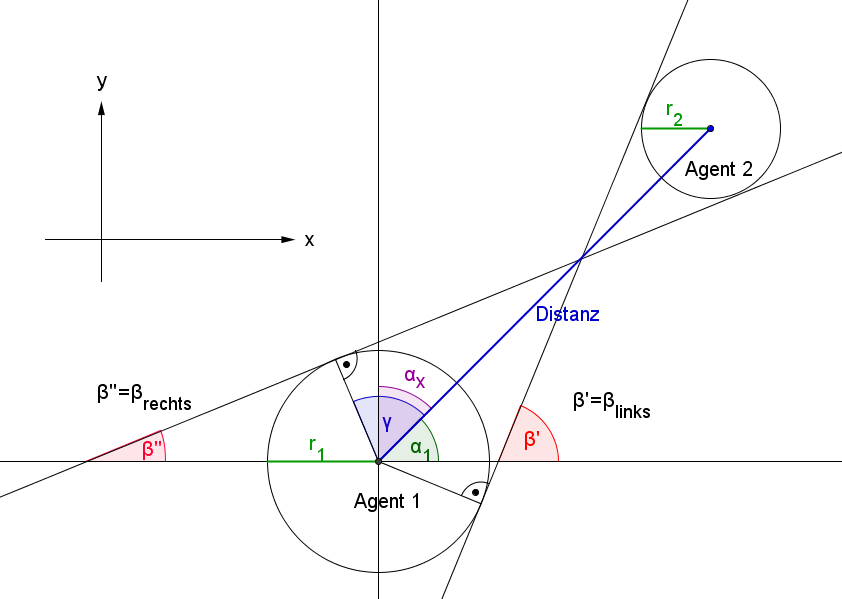
\includegraphics[width=0.80\textwidth]{pictures/beta.PNG}
	\caption{The graph shows the angles and variables used to get $\beta_\y{Links}$ and $\beta_\y{Rechts}$. $\alpha_X$ is the angle between the two agents with respect to the $y$-axis. This depiction was engineered to work also for agents walking the other way.}
	\label{fig:beta}
\end{figure}

\noi For our model, it is crucial to determine where an agent shouldn't go. The function \textit{getBeta.m} returns the angles which describe the interval of angles leading to a collision. A graphical depiction of the situation is given in figure \ref{fig:beta}. The equations (\ref{logik3}) to (\ref{logik5}) were used to get $\beta_\y{Links}$ and $\beta_\y{Rechts}$. They had to be converted into the angles given with respect to $\varphi$, $\beta_{\varphi,\y{ left}}$ and $\beta_{\varphi,\y{ right}}$ as shown in equations (\ref{logik6}) to (\ref{logik7}).
\begin{equation}\label{logik3}
	\gamma = arccos\brac{\frac{r_S}{d}},\ \alpha = arctan\brac{\frac{\Delta y}{\Delta x}}
\end{equation}
\begin{equation}\label{logik4}
	\beta_\y{Links} = \gamma + \alpha - \frac{\pi}{2}
\end{equation}
\begin{equation}\label{logik5}
	\beta_\y{Rechts} = \alpha + \frac{\pi}{2} - \gamma
\end{equation}
\begin{equation}\label{logik6}
  \beta_{\varphi,\y{ left}} = \frac{\pi}{2} - \beta_\y{Links} = \pi - (\gamma + \alpha)
\end{equation}
\begin{equation}\label{logik7}
  \beta_{\varphi,\y{ right}} = \frac{\pi}{2} - \beta_\y{Rechts} = \gamma - \alpha
\end{equation}
\noi This works between agents as well as between agents and the wall agents. Care was taken to engineer a calculation that allows for it to be used for agents walking in both directions.

\subsubsection{Calculation of the interaction with another dynamic agents}
\text{xValuesLogic.m} distinguishes three different cases.
\begin{itemize}
	\item For two crossing agents or if the agent in front of the agent in question is slower, we used equation (\ref{logik1}) to get $x_\y{out}'$. It was also used for two not moving agents, setting $\Delta v$ equal to an arbitrary value given in \texttt{STANDOFF}. This was a quick way to resolve standoffs, although this would eventually turn out to be in its actual form an Achilles heel of the model.
	\begin{equation}\label{logik1}
		x_\y{out}' = \frac{1}{\dis (|x - \alpha_X|)^{\brac{\frac{-\Delta v}{a}}}} = (|x - \alpha_X|)^{\brac{\frac{\Delta v}{a}}},\ \Delta v < 0
	\end{equation}
	\noi All values which correspond to a collision course in $x_\y{out}'$ are set to zero. This also deals with the singularity of equation (\ref{logik1}) as it is set to zero. This is done using the $\beta$-angles shown before. Afterwards, $x_\y{out}'$ is normalized and modificated further using equation (\ref{logik2}).
	\begin{equation}\label{logik2}
		x_\y{out} = x_\y{out}' \cdot \frac{b}{max(x_\y{out}')} \cdot \brac{\frac{r_S}{d}}^c
	\end{equation}
	\noi The variables $a$ (called \texttt{SLOPEFACTOR}), $b$ (\texttt{HEIGHT}) and $c$ (\texttt{REPULSIONAGENT}) have to chosen in a way that the simulation runs smoothly. The term $\frac{b}{max(x_\y{out}')}$ normalized the function to a maximum value $b$ while the term $\brac{\frac{r_S}{d}}^c$ controls that the repulsive influence gets stronger, the closer the two agents get. $c$ is usually chosen to be larger than 1.\\
	For two agents walking the in the same direction, the function given in equation \ref{logik2} is additionally multiplied with the difference in speed $|\delta v|$ in a try to make them avoid standing agents more resolute as it that case $|\delta v|$ would be rather big.\\
	
	\noi If the $x_\y{out}$ given in equation (\ref{logik2}) would be returned, the agent in question would aim to miss the other agent exactly. We thought that this would be too close as in reality, one also leaves a bit of space if possible between each other. Therefore we introduced an offset given as \texttt{WALLANGLEOFFSET} which gives the angle additionally to the $\beta$ angles for which an agent should aim to. To account for this, $x_\y{out}$ is modified with an linear interpolation between the values at $\beta + $\texttt{WALLANGLEOFFSET} and $\beta$ (which was set to zero before).

	\item If the agent in front of the agent in question is faster, a gaussian curve was used with the mean $\alpha_X$ and standard deviation $rS/d$. It is then modified further with $\Delta v$ and \texttt{HEIGHT} to make it a weak influence.
	\item For two agents moving with the same speed, the influence is set to zero by returning a vector of zeros.
\end{itemize}


\subsubsection{Calculation of the interaction with a wall agents}
To avoid hitting the wall, we used a very simple approach. Every angle corresponding to a collision course is set to a negative value accoring to equation (\ref{logik8}).
\begin{equation}\label{logik8}
	x_\y{Out} = x \cdot \frac{a}{d - rS}
\end{equation}
\noi As before for agents, an offset is introduced so the agent in question doesn't just try to avoid the wall-agent but also to leave some buffer space. The offset is also given in \texttt{WALLANGLEOFFSET}, $a$ can be accessed with the constant variable \texttt{WALLFACTOR}. $a$ has to be set negative as otherwise the wall would have an attracting force. To set a good value for this factor $a$ is quite delicate because if it is too low, agents will be stuck in the wall while if it too high, they will never approach the wall even slightly. 

\pagebreak
\subsubsection{Calculating functions in $x$ and transforming them into a polar axis in $\varphi$}
\begin{figure}[h!]
	\centering
		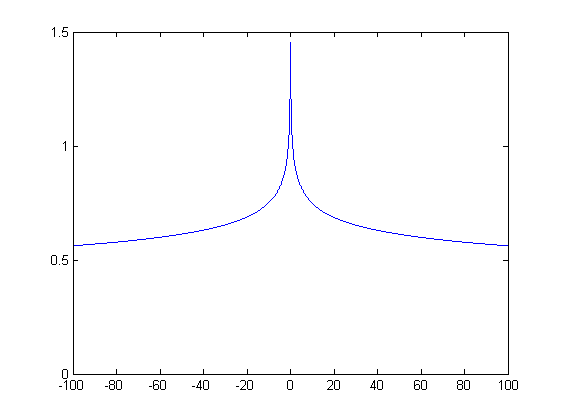
\includegraphics[width=0.40\textwidth]{pictures/Bsp2}
		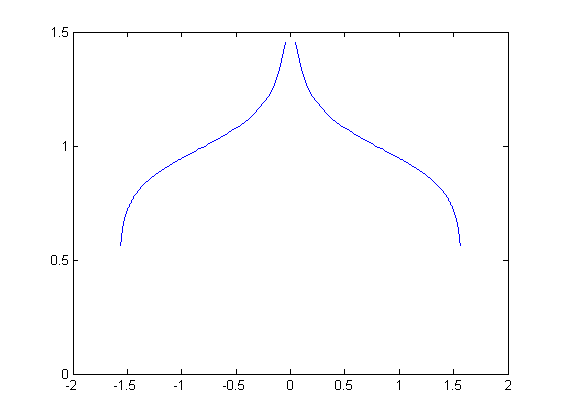
\includegraphics[width=0.40\textwidth]{pictures/Bsp2Angle}
	\caption{Graphical depiction of the function given in equation (\ref{logik1}). In the graphic on the left, the horizontal axis is given in $x$ while in the right graphic the horizontal axis is given in $\varphi$.}
	\label{fig:Bsp2}
\end{figure}

\noi As the functions given above are given in $x$ but the direction to go on is determined in polar values, it needs to be transformed into a $\varphi$ axis. This is done using a vector for $x$ ranging $\pm$ \texttt{XSCOPE} with a step of \texttt{XRES}. Applying the arcustangent on it yields the axis in angular values ($\varphi$). The transforming is done simply by using the $\varphi$ axis instead of the $x$ axis. This is shown in the two figures \ref{fig:Bsp2} and \ref{fig:Bsp2Out}. As those functions are only chosen to show the principle, they were not normalized in height according to the equations mentioned above.\\
\begin{figure}[h!]
	\centering
		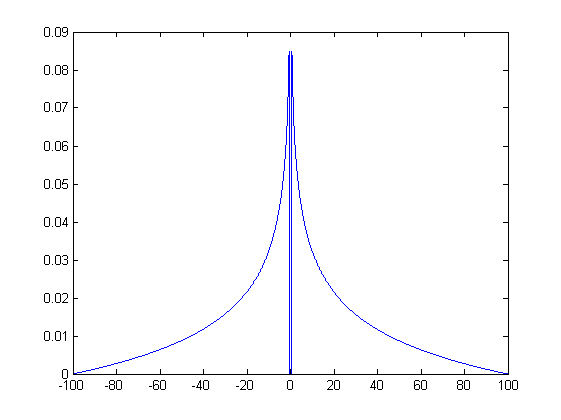
\includegraphics[width=0.40\textwidth]{pictures/Bsp2Out}
		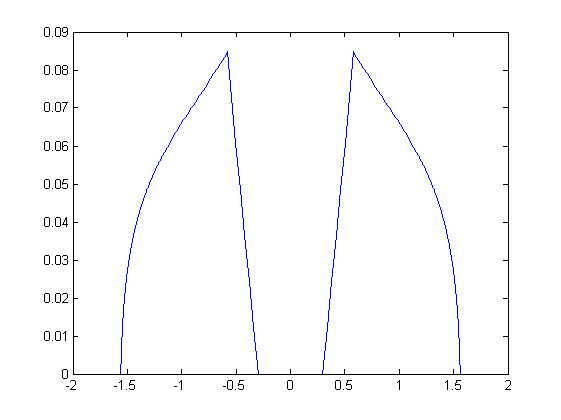
\includegraphics[width=0.40\textwidth]{pictures/Bsp2OutAngle}
	\caption{Graphical depiction of the return values of the function \textit{xValuesLogic.m}. In the graphic on the left, the horizontal axis is given in $x$ while in the right graphic the horizontal axis is given in $\varphi$. $\alpha_X$ was set to 0 corresponding to an other agent directly ahead, $\beta$ was set to $\pm 0.3$ with an offset of $0.25$.}
	\label{fig:Bsp2Out}
\end{figure}

In figure \ref{fig:Bsp2}, the function (\ref{logik1}) is shown graphically in the $x$ as well as $\varphi$ axis. Figure \ref{fig:Bsp2Out} shows the $x_\y{out}$ the function \textit{xValuesLogic.m} returns.



\subsubsection{Graphical example}
This subchapter shall give a visual example of how the logic functions work. Let's consider the situation given in figure \ref{fig:Bsp1}.
\begin{figure}[h!]
	\centering
		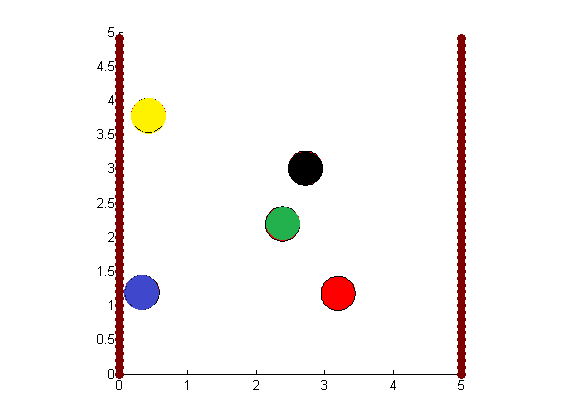
\includegraphics[width=0.45\textwidth]{pictures/Bsp1}
	\caption{Exemplary case used to demonstrate the working principle of the logic functions.}
	\label{fig:Bsp1}
\end{figure}

\noi The blue agent moving up in figure \ref{fig:Bsp1} only sees the influence of the wall. What the blue agent "sees" is given in figure \ref{fig:Bsp1LinksUnten}. The influence of the wall causes the overall function to decrease for all $\varphi$ corresponding to a collision course. The offset causes the overall function to have its maximum $\alpha$ at a positive $\varphi$. This causes the agent to walk in the direction of $\alpha$.\\
\begin{figure}[h!]
	\centering
		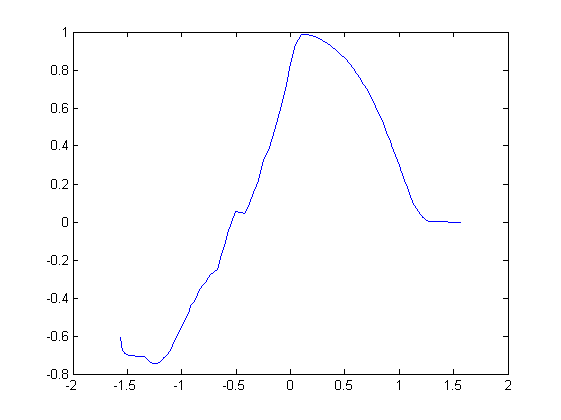
\includegraphics[width=0.4\textwidth]{pictures/Bsp1LinksUnten}
	\caption{Output of all logic functions combined for the blue agent in figure \ref{fig:Bsp1}. Visible is the effect of wall agents on the blue agent as negative values on the left side.}
	\label{fig:Bsp1LinksUnten}
\end{figure}

\noi The green agent moving up sees only the influence of the black agent who is moving down. The effect of that it given in figure \ref{fig:Bsp1Mitte}. The underlying gaussian function can be seen as well as the addition of a modified version of figure \ref{fig:Bsp2Out}, left. The agent will move slightly to the left to avoid hitting the black agent.\\
\begin{figure}[h!]
	\centering
		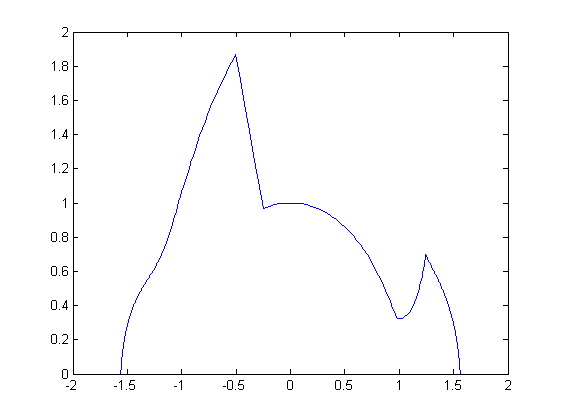
\includegraphics[width=0.40\textwidth]{pictures/Bsp1Mitte}
	\caption{Output of all logic functions combined for the green agent in figure \ref{fig:Bsp1}. Visible is the effect of the oncoming black agent as a superposition on the underlying gaussian curve.}
	\label{fig:Bsp1Mitte}
\end{figure}

\noi The black agent moving down sees the oncoming green and red agent going up. The effect of them is given in figure \ref{fig:Bsp1ObenRechts}. The superposition of two functions onto the underlying gaussion can be seen by the discontinities. The effect of the green agent is stronger as it is nearer to the black agent than the red agent which causes the black agent to go left (looking top-down) in order to avoid hitting the green agent. This shows the dependency of the strength of an agent of the distance.
\begin{figure}[h!]
	\centering
		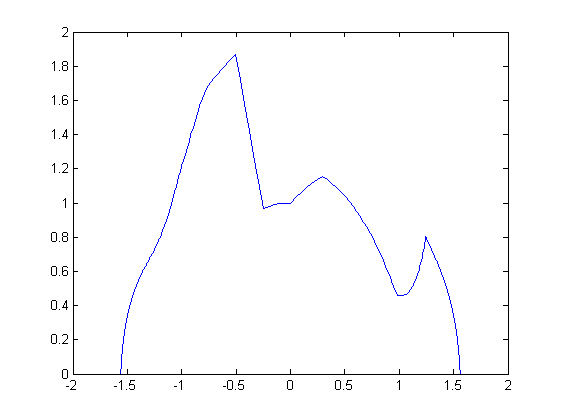
\includegraphics[width=0.40\textwidth]{pictures/Bsp1ObenRechts}
	\caption{Output of all logic functions combined for the black agent in figure \ref{fig:Bsp1}. Visible is the effect of the oncoming green and red agents as superpositions on the underlying gaussian curve. The black agent will move left (from his point of view) to avoid hitting the closer green agent.}
	\label{fig:Bsp1ObenRechts}
\end{figure}
